\documentclass[tikz,border=10pt]{standalone}
\usepackage{tikz}
\usetikzlibrary{arrows.meta,positioning,calc}
\begin{document}
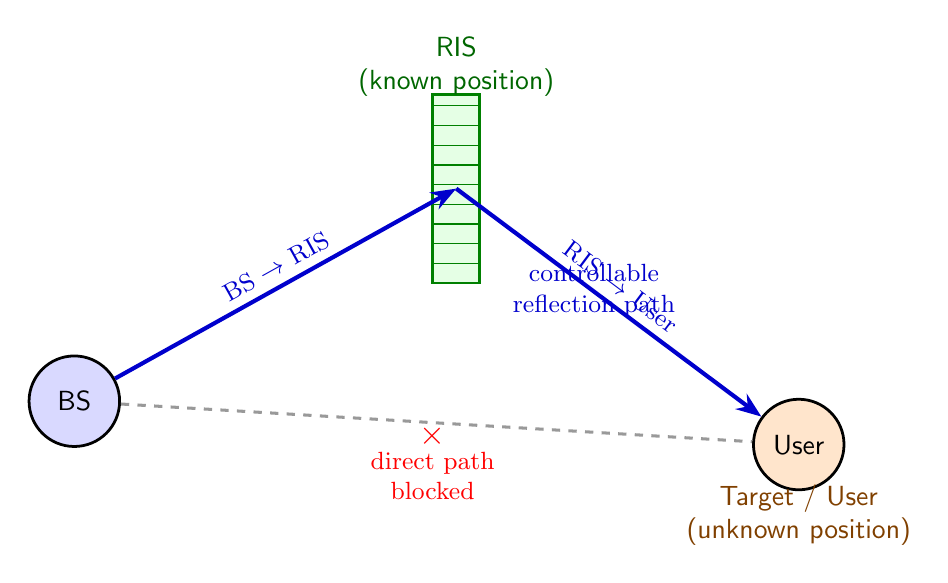
\begin{tikzpicture}[font=\sffamily,>=Stealth]
  % Base station
  \node[draw, circle, fill=blue!15, minimum size=1.15cm, line width=1pt] (bs) at (-4.8,0) {BS};

  % RIS panel
  \draw[fill=green!10, draw=green!50!black, line width=1pt] (-0.25,1.5) rectangle (0.35,3.9);
  \foreach \y in {1.75,2.0,...,3.75} {
    \draw[green!50!black] (-0.25,\y) -- (0.35,\y);
  }
  \node[align=center, text=green!40!black] at (0.05,4.25) {RIS\\(known position)};

  % User
  \node[draw, circle, fill=orange!20, minimum size=1.15cm, line width=1pt] (user) at (4.4,-0.55) {User};
  \node[align=center, text=orange!50!black] at (4.4,-1.45) {Target / User\\(unknown position)};

  % Blocked direct path
  \draw[dashed, gray!80, line width=1.1pt] (bs) -- (user);
  \node[red, font=\bfseries\large] at (-0.25,-0.45) {$\times$};
  \node[red, align=center, font=\small] at (-0.25,-0.95) {direct path\\blocked};

  % Reflected path
  \draw[-{Stealth[length=3.2mm]}, blue!80!black, line width=1.5pt]
        (bs) -- node[midway, above, sloped, font=\small] {BS $\rightarrow$ RIS} (0.05,2.7);
  \draw[-{Stealth[length=3.2mm]}, blue!80!black, line width=1.5pt]
        (0.05,2.7) -- node[midway, above, sloped, font=\small] {RIS $\rightarrow$ User} (user);

  \node[blue!80!black, align=center, font=\small] at (1.8,1.4) {controllable\\reflection path};
\end{tikzpicture}
\end{document}
